\chapter{Introduction}

\label{Chapter1} % For referencing the chapter elsewhere, use \ref{Chapter1} 

La présentation de projets d'urbanisme ou de planification territoriale auprès du public a toujours été un défi. 

Depuis son apparition, la CAO aide les professionnels du domaine à réaliser des modélisations toujours plus précises et réalistes. 
Malheureusement, pour partager ces réalisations, cela nécessite généralement de réaliser des maquettes 3D soi-même. Cela demande d'autant plus de travail et de temps que le projet est complexe, voire inclut différentes étapes (2 ans, 5 ans...), auquel cas plusieurs versions de maquettes sont à réaliser.

\begin{figure}[h]
    \centering
    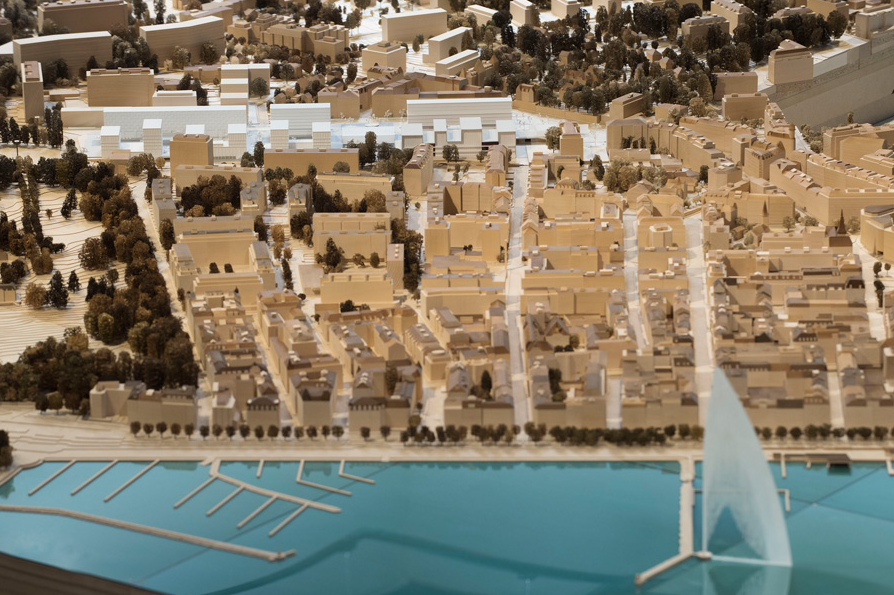
\includegraphics[width=0.8\linewidth]{Figures/geneva-model.png}
    \caption{Maquette de la ville de Genève réalisée à la main}
    \label{fig:geneva-model}
\end{figure}

L'avènement des imprimantes 3D a permis de réduire cette charge de travail, tout en produisant des maquettes plus fidèles. 


\begin{figure}[h]
    \centering
    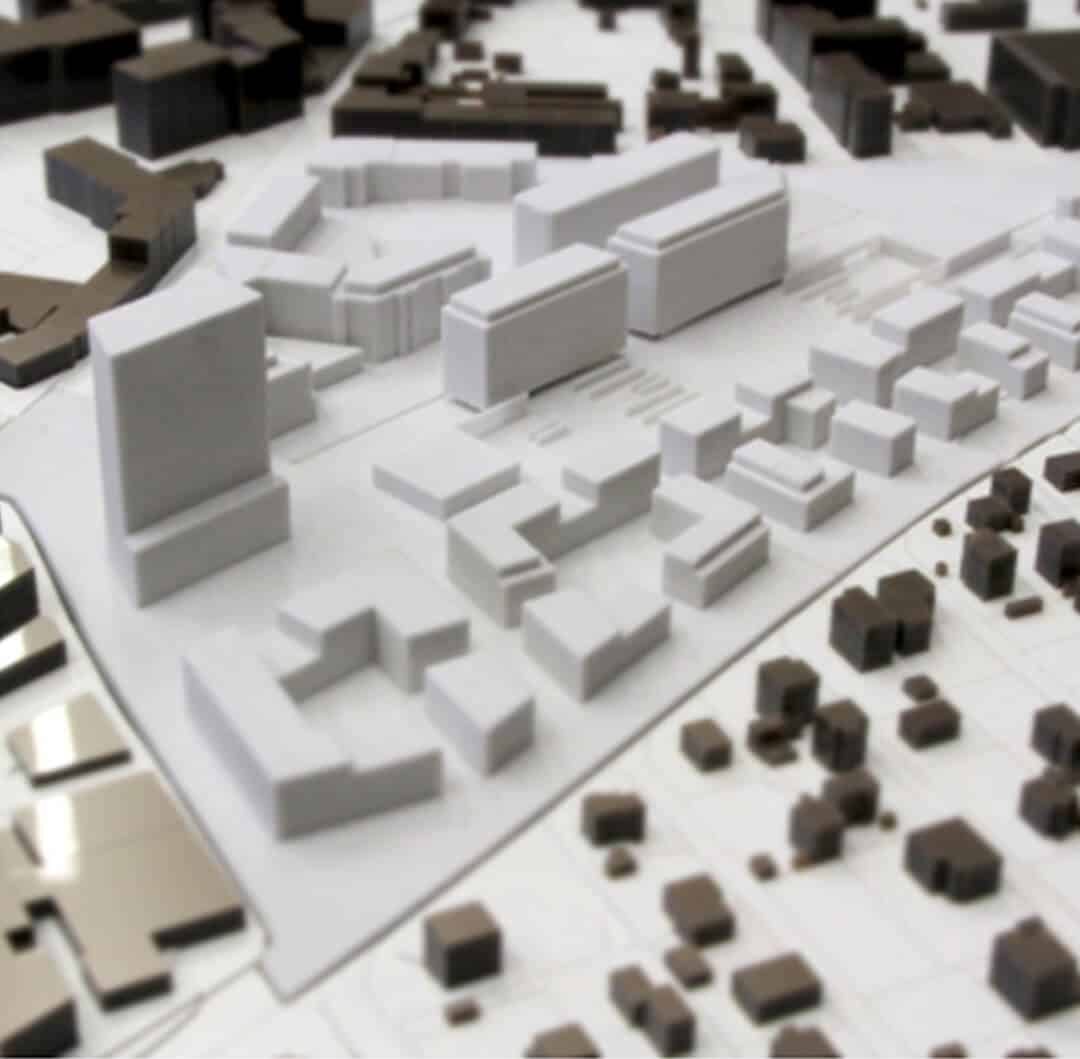
\includegraphics[width=0.5\linewidth]{Figures/3dprinted-model.jpg}
    \caption{Exemple de maquette imprimée en 3D}
    \label{fig:3dprinted-model}
\end{figure}

Dans tous les cas, un autre problème est là : pour voir lesdites maquettes, il faut se rendre à l'endroit où elles sont exposées.

Une solution à cela serait de partager directement les modèles réalisés à l'ordinateur auprès des personnes concernées. Cependant, la majorité des projets sont réalisés à l'aide de logiciels propriétaires, et dont la licence est bien souvent très coûteuse (AutoCAD, SketchUp, Cinema4D...). Il n'est dès lors pas envisageable d'exiger des utilisateurs un tel investissement d'argent et de temps (installation, configuration) dans un simple but de consultation des projets réalisés.
Certes, certains de ces produits proposent gracieusement une visionneuse, mais celle-ci est généralement limitée aux formats supportés par l'éditeur.

Fort heureusement, des outils gratuits permettant de visualiser des modèles 3D de toutes sortes onf fait leur apparition sur le marché ces dernières années. Certains sont proposés gracieusement par les éditeurs des produits tels que cités précédemment, à l'instar d'Autodesk Viewer. D'autres sont des logiciels clients, comme la visionneuse 3D fournie d'office avec Windows 10 ou Open 3D Model Viewer\footnote{\url{www.open3mod.com}}. Enfin, des solutions en ligne sont également disponibles. Celles-ci ont l'avantage de ne nécessiter aucune installation, et d'être accessibles à la majorité des systèmes d'exploitation, ne nécessitant qu'un navigateur internet.
C'est cette dernière catégorie qui nous intéresse dans le cadre de ce projet.

Parmis les outils en ligne existants, le plus utilisé, et sans doute le plus complet actuellement, se nomme \textbf{Sketchfab}. Plus qu'une simple visionneuse, il s'agit d'une plateforme permettant de stocker, partager et visualiser des modèles 3D. Elle sera détaillée dans la section \ref{sketchfab}.

\section{Sketchfab} \label{sketchfab}

Lancée en 2012, Sketchfab\footnote{\url{www.sketchfab.com}} est une plateforme web d'hébergement de contenus 3D, ne ciblant aucune catégorie particulière : cela va des modèles de petits objets de la vie courante, de personnages, aux modélisations de paysages et lieux complexes.

\begin{figure}
    \centering
    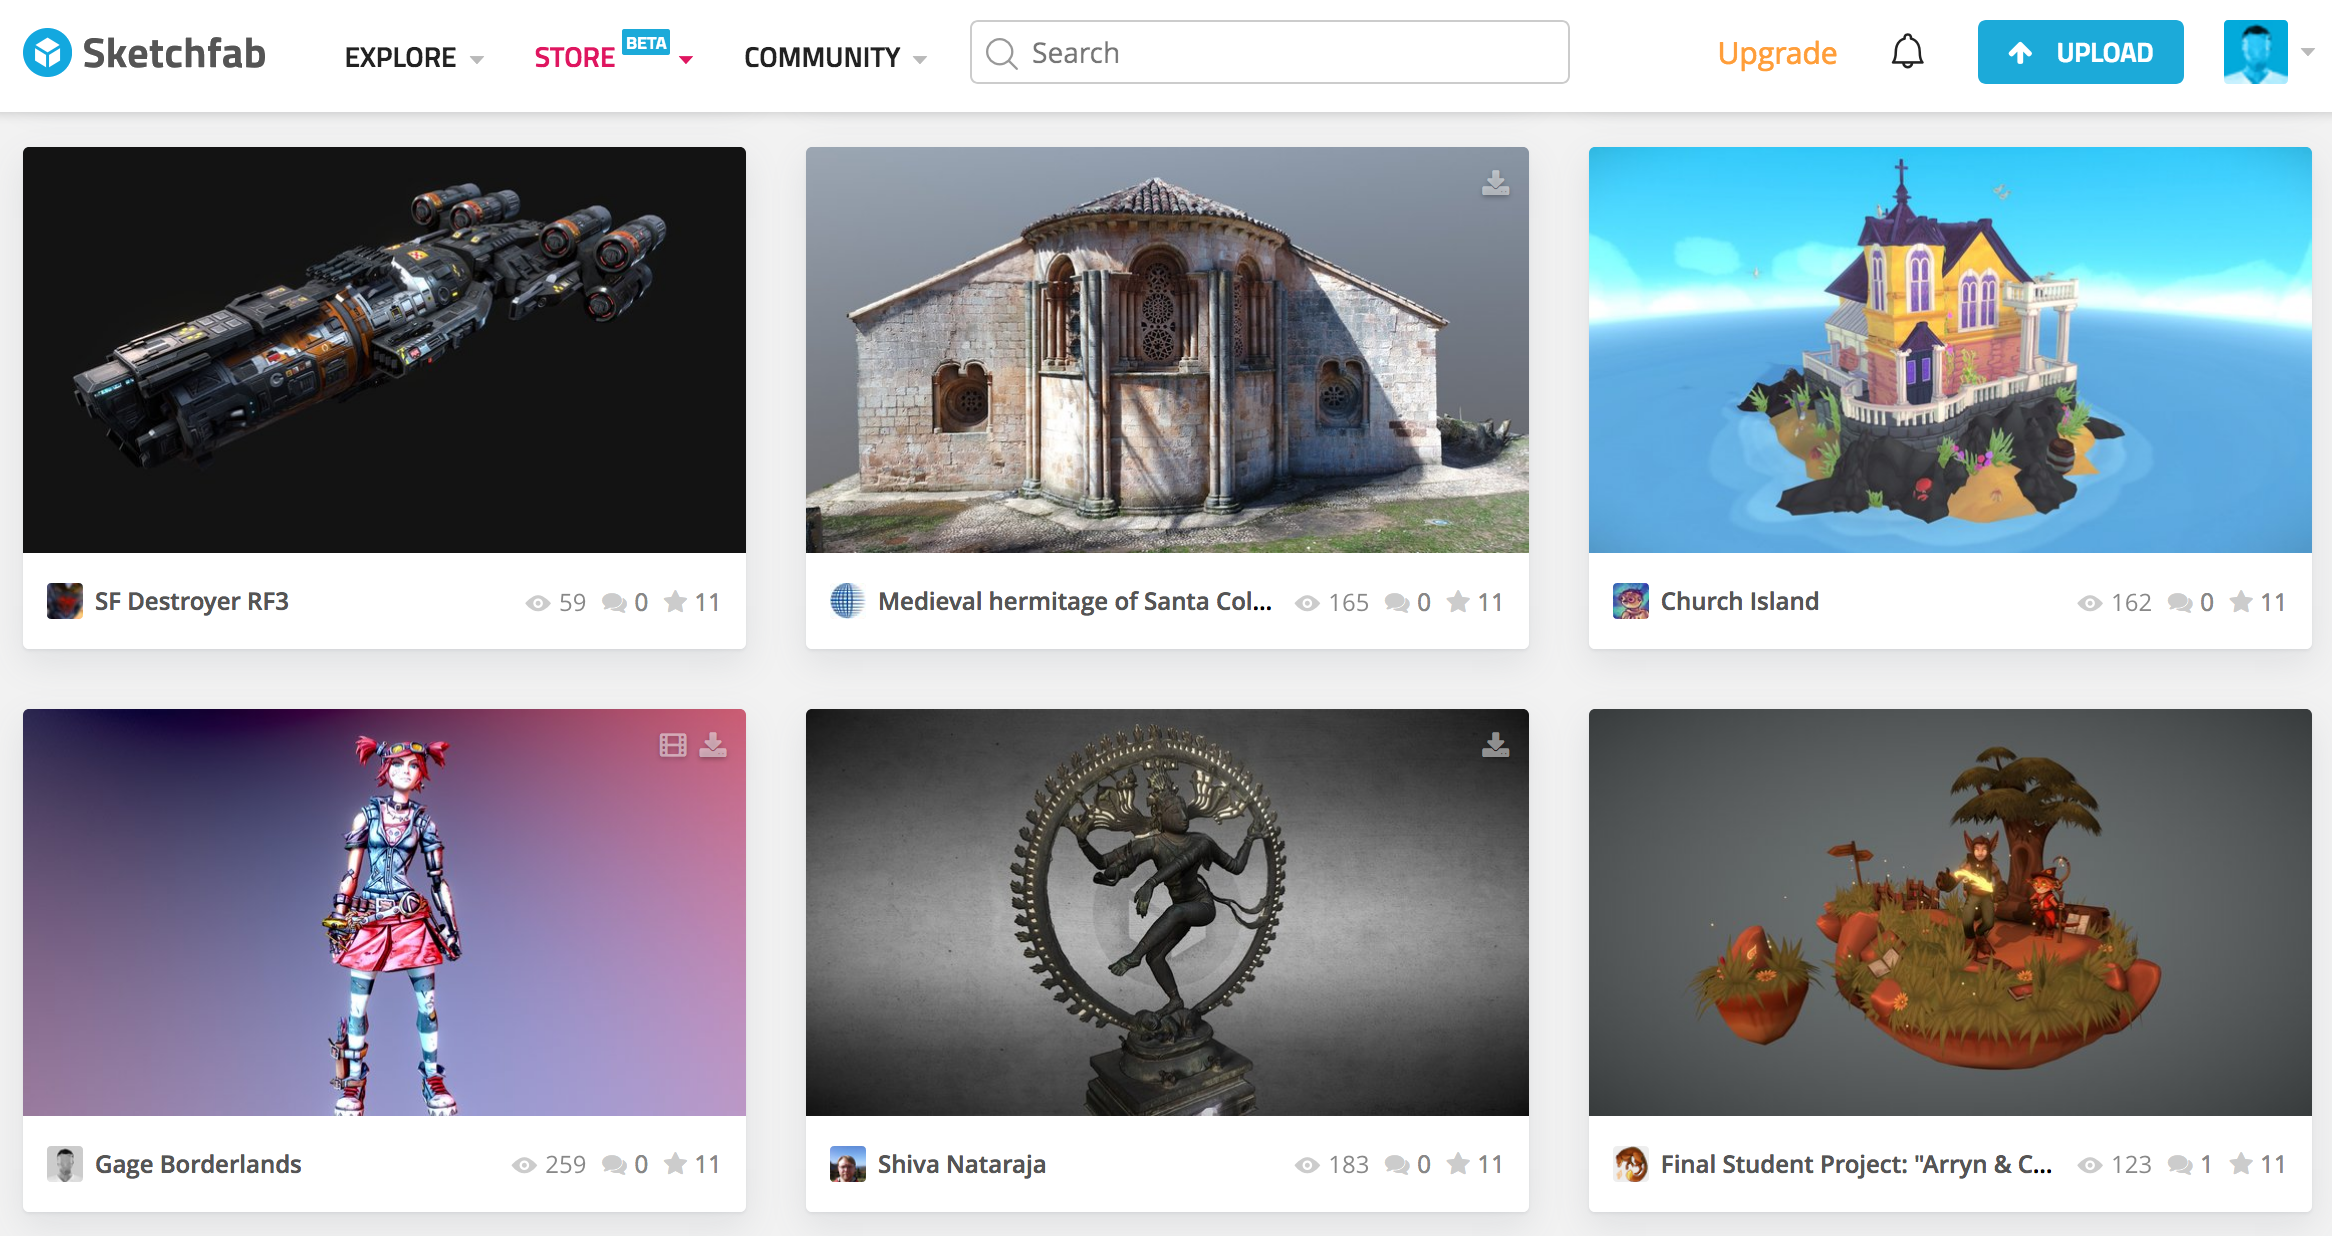
\includegraphics[width=\linewidth]{Figures/sketchfab-overview.png}
    \caption{Affichage de modèles récemments ajouté à Sketchfab}
    \label{fig:sketchfab-overview}
\end{figure}

Elle permet de visualiser les modèles 3D sur toutes plateformes possédant un navigateur (ordinateurs, smartphones, et même casques de réalité virtuelle).
Il est ainsi possible de naviguer dans le modèle à l'aide d'une souris ou de manière tactile, selon le support. Les opérations "classiques" telles que \textit{zoomer} ou \textit{pivoter} sont disponibles.
Le propriétaire d'un modèle peut également lui adjoindre des annotations. Une annotation est liée à une coordonnée 3D choisie sur le modèle, possède un titre, et peut contenir un texte descriptif ou une image.

\begin{figure}[ht]
    \centering
    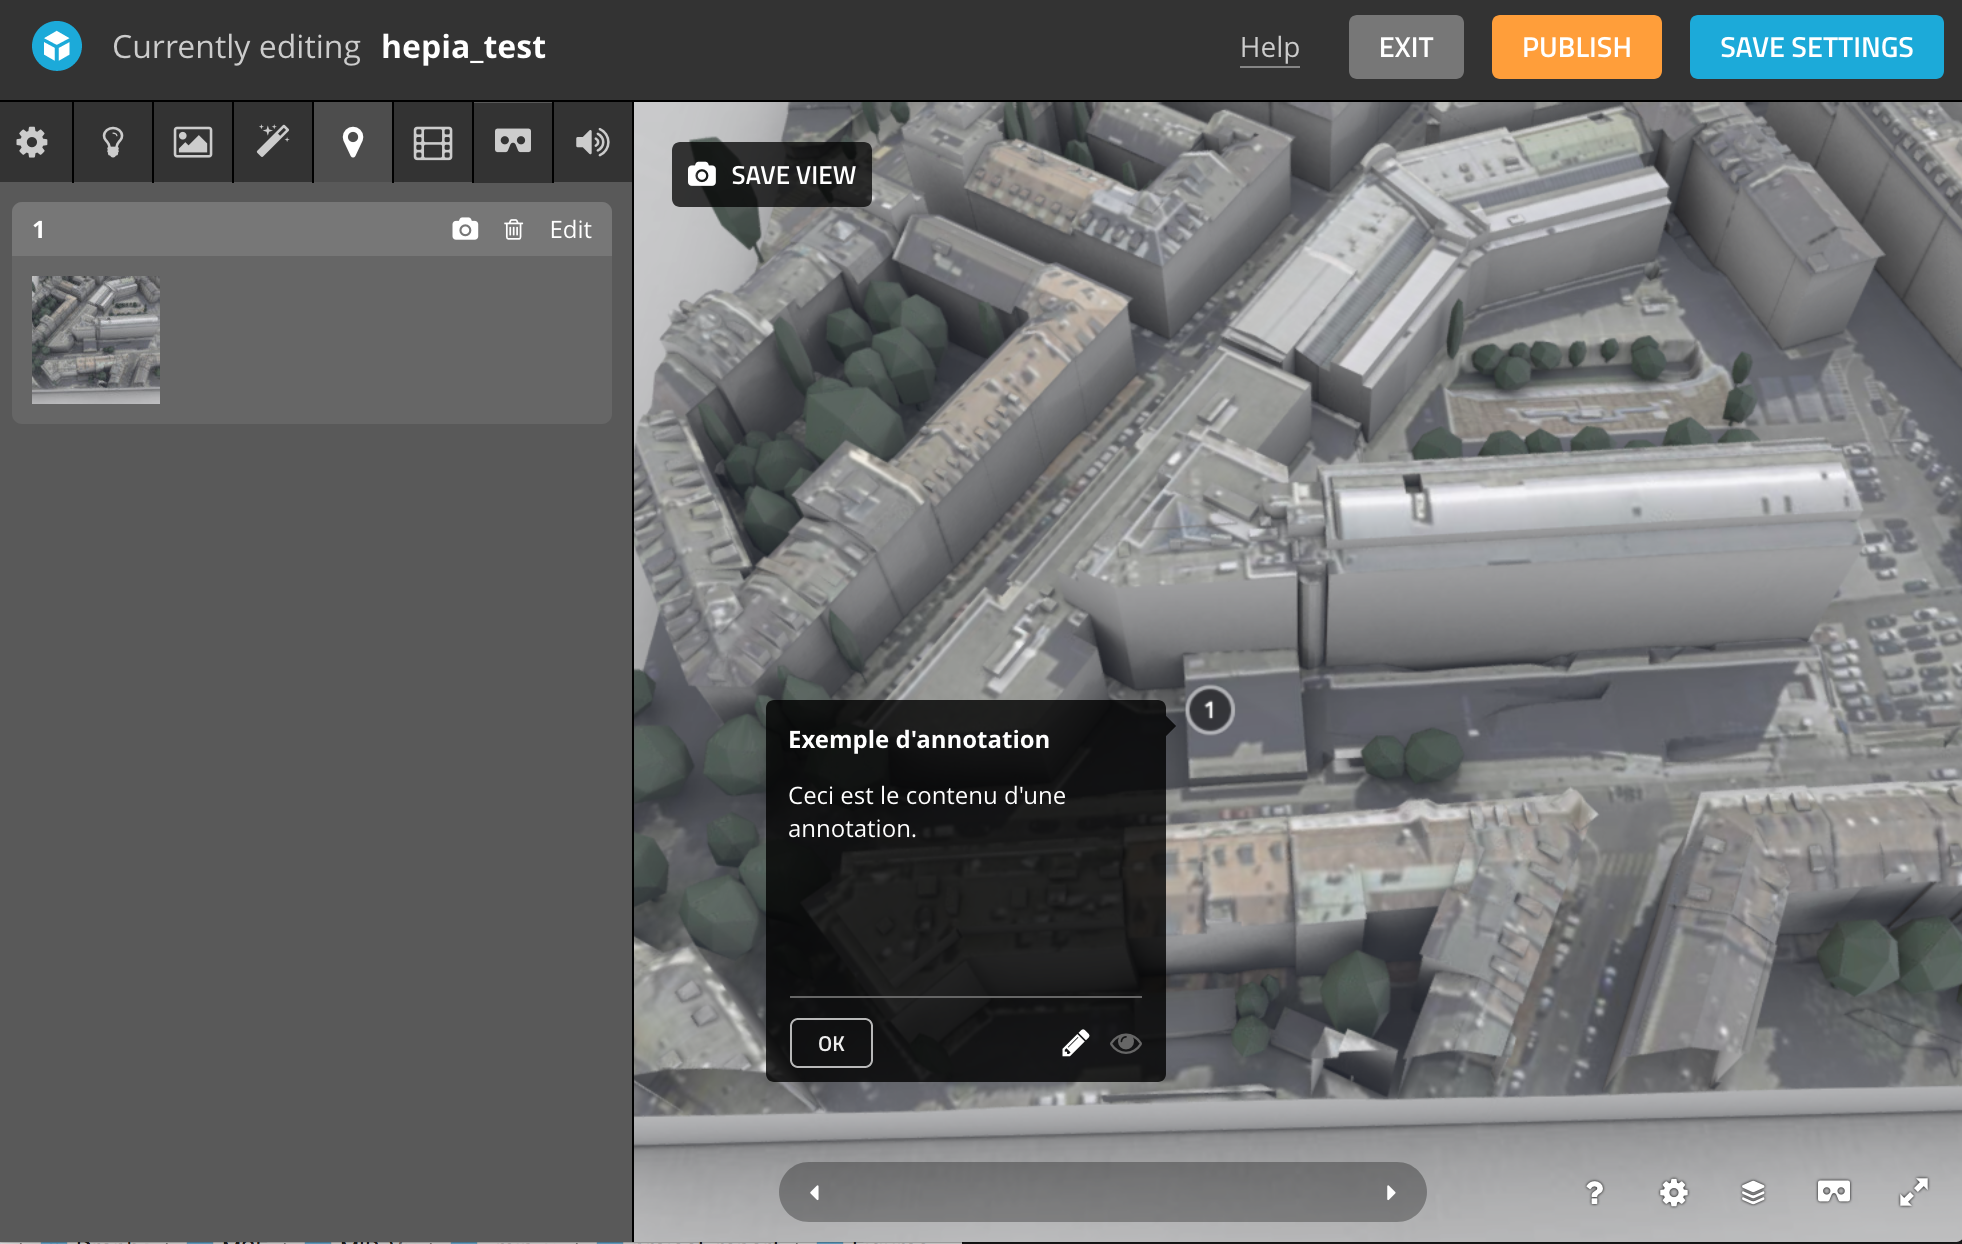
\includegraphics[width=\linewidth]{Figures/sketchfab-annotation-example.png}
    \caption{Ajout d'une annotation à un modèle dans Sketchfab}
    \label{fig:sketchfab-annotation-example}
\end{figure}

Sketchfab propose plusieurs niveaux de fonctionnalités \footnote{\url{https://sketchfab.com/plans}}. Les principales limitations de l'offre gratuite sont :
\begin{itemize}
    \item Les modèles ajoutés sont obligatoirement référencés et publiques; il n'est pas possible d'en restreindre l'accès,
    \item La taille maximale d'un modèle est de 50 Mo, contre plusieurs centaines de Mo avec une offre payante, ce qui est assez restreignant,
    \item Seules 5 annotations peuvent être ajoutées à un modèle
\end{itemize}

Récemment, la plateforme a mis en place un \textit{store} (encore en version \textit{beta}) permettant de vendre et acheter des modèles, généralement un peu plus complexes et travaillés.

\section{Réalisation}
\todo{faire apparaître "architecture composants" dans objectifs}

\section{Problématique}

À la Haute école du paysage, d'ingénierie et d'architecture de Genève (hepia), le groupe de modélisation informatique du paysage\footnote{\url{mip.hesge.ch}} (MIP) perçoit l'intérêt que présente un tel outil dans le cadre de ses mandats. En intégrant une telle plateforme dans son flux de travail, le partage et l'accès aux modélisations auprès des acteurs concernés s'en trouverait facilité.

\textit{Sketchfab} présente néanmoins des lacunes. Pour commencer, les limitations évoquées dans la section \ref{sketchfab}, bien que pouvant être plus ou moins résolues en optant pour une formule payante.
S'agissant d'une plateforme généraliste, elle n'offre pas forcément certains outils spécifiques, propres au domaine de l'urbanisme. D'autres inconvénients, comme le manque de personnalisation (par exemple, pouvoir isoler les modèles concernant un projet), les droits d'accès (gérer les personnes autorisées à consulter un groupe de modèles, ainsi que les possibilités d'interactions de chacun).


\todo{Limitations des annotations : \url{https://help.sketchfab.com/hc/en-us/articles/202512456-Annotations?utm_source=website&utm_campaign=plans_page}}

Idéalement, il faudrait pouvoir bénéficier d'une plateforme similaire à \textit{Sketchfab}, mais répondant aux besoin spécifiques du domaine de l'aménagement du territoire, en offrant la possibilité d'être aisément personnalisable à cet effet.

\section{Objectifs}

\todo{Où et comment mentionner Oliver Donzé, le MIP, etc... ?}
Le but du présent projet est d'établir la faisabilité de réalisation et mise en place d'une telle plateforme à vocation collaborative.

Un projet d'approfondissement s'effectue sur un temps relativement restreint. 
Par conséquent, l'accent est mis sur :


\begin{itemize}
    \item Définir l'architecture de la plateforme,
    \item Déterminer et présenter des cas d'utilisation,
    \item Rechercher et étudier les solutions existantes qui pourraient servir à composer les différentes "briques" du logiciel,
    \item Etudier les technologies de visualisation de maquettes numériques 3D
    \item Réaliser, si possible, un prototype ou des illustrations à des fins démonstratives
\end{itemize}

